\section{补充实验}
\label{app:historical_diagnostics}

本节给出早期方法结果、过滤器和选择器的完整测试、首次收据测试、解析细节与补充检查。主要结果见第~\ref{sec:experiments}~节。

% Begin merged sections/historical_pipeline.tex
\subsection{早期方法与过滤测试}
\label{sec:eval:ablation}

表~\ref{tab:repair_ablation}~比较四种已保存设置。不使用模型补全时返回清理后的图。直接调用模型 使用自己的提示，并跳过清理。过滤测试对同一建议在检查前后计分。第~\ref{sec:eval:mechanisms}~节测试提示文本，第~\ref{sec:eval:individual_ablation}~节测试过滤器和选择器的各个步骤。

\begin{table}[t]
\centering
\caption{注入缺陷输入上的四种设置。直接调用模型使用不同提示。}
\label{tab:repair_ablation}
\small
\begin{tabular}{l c c c c}
\toprule
变体 & 修复率 & 过度修复 & F1 & 精确匹配 \\
\midrule
无模型补全 & 0.3200 & 0.0000 & 0.8472 & 0.0622 \\
直接调用模型（独立提示） & 0.9244 & 0.0758 & 0.9520 & 0.8267 \\
无约束门控 & 0.9800 & 0.0227 & 0.9895 & 0.9333 \\
\textbf{诊断＋门控} & \textbf{0.9800} & \textbf{0.0167} & \textbf{0.9917} & \textbf{0.9333} \\
\bottomrule
\end{tabular}
\end{table}

模型补全恢复大多数缺失字段。诊断＋门控 的 F1 为 99.17\%，直接调用模型 为 95.20\%。过滤保持相同修复率，并使过度修复降低 0.60 个百分点。它去掉八条未通过来源匹配的三元组，均与参考不同。

% Begin merged sections/ablation_offline.tex
\subsection{过滤器与选择器步骤测试}
\label{sec:eval:individual_ablation}

我们使用共享提示测试中的 360 个 Gemma 响应，以及新收据测试中的 180 个响应。每个响应经过八种过滤设置：全部检查、分别去掉五项检查中的一项、同时去掉重复与字段数量检查，以及去掉全部检查。540 个响应得到 4,320 个评分输出，候选顺序保持固定。同时去掉两项检查，用于测试两者如何相互影响。

表~\ref{tab:gate_checks}~给出完整过滤器的 F1 减去改变后过滤器的 F1。先对同一文档的三个提示取平均，再对文档取平均。完整过滤器拒绝 28 条三元组，其中 11 条文档编号错误，17 条来源匹配失败，均与参考不同。其他检查未额外去掉候选。模型构建输入中，来源匹配增加 0.505 个 F1 百分点，编号检查增加 0.085 个百分点。21 项校正后的检验 $p$ 值均大于 0.05。日志也列出移除某项检查后丢失的正确事实。

\begin{table}[t]
\centering
\caption{各项过滤检查带来的 F1 变化，单位为百分点。每组输入有 60 篇文档和三种提示。正值表示完整过滤器更好。}
\label{tab:gate_checks}
\small
\begin{tabular}{lrrr}
\toprule
移除的检查 & 受控输入 & 模型构建输入 & 收据 \\
\midrule
重复 & +0.000 & +0.000 & +0.000 \\
文档头节点 & +0.037 & +0.085 & +0.000 \\
关系类型 & +0.000 & +0.000 & +0.000 \\
来源支持 & +0.037 & +0.505 & +0.060 \\
字段数量 & +0.000 & +0.000 & +0.000 \\
重复＋字段数量 & +0.000 & +0.000 & +0.000 \\
全部检查 & +0.073 & +0.590 & +0.060 \\
\bottomrule
\end{tabular}
\end{table}

% Begin merged sections/v2_ablation.tex
\paragraph{当前编辑选择器测试。}

我们在 225 个注入缺陷输入和 225 个模型构建输入的保存建议上运行 v2 选择器。13 种设置在默认绝对先验评分下产生 5,850 个结果，再用相对等权重评分重复测试，得到另外 5,850 个结果。两次均使用 \texttt{public-profile-v2} 特征和重新训练的路由器。档案保留较早的 v1 运行。

基础设置使用等权重，并让选择器始终开启。每个测试改变一个指定步骤。触发器测试从始终开启的学习权重设置开始。去掉某项分数时，将该项置零，并去掉对应边界，其他权重不变。规则检测器和违规减少奖励继续使用。去掉规则候选时，移除检测器动作和直接来源字段添加；图评估概况与保存的模型建议继续使用。

\begin{table}[t]

\centering

\caption{默认绝对先验评分下的 v2 选择器。接受数统计动作或编辑包，按注入缺陷／模型构建输入排列。每项 F1 使用 225 篇文档。}
\label{tab:optimizer_complete}

\small

\begin{tabular}{lrrr}

\toprule

设置 & 受控 F1 & 模型构建 F1 & 接受数 \\

\midrule

始终开启、均匀先验 & 0.8472 & 0.8833 & 0 / 10 \\

学习先验、始终开启 & 0.8472 & 0.8799 & 0 / 10 \\

学习先验与触发器 & 0.8472 & 0.8799 & 0 / 10 \\

无先验惩罚 & 0.8472 & 0.8833 & 0 / 10 \\

无动作成本 & 0.8930 & 0.8813 & 68 / 13 \\

无密度上界 & 0.8472 & 0.8833 & 0 / 10 \\

无质量下界 & 0.8472 & 0.8833 & 0 / 10 \\

仅一轮 & 0.8472 & 0.8833 & 0 / 10 \\

无规则候选 & 0.8472 & 0.8833 & 0 / 9 \\

仅规则候选 & 0.8472 & 0.8799 & 0 / 10 \\

无局部分数及边界 & 0.8472 & 0.8799 & 0 / 0 \\

无图分数及边界 & 0.8472 & 0.8833 & 0 / 10 \\

无来源分数及边界 & 0.8472 & 0.8799 & 0 / 10 \\

\bottomrule

\end{tabular}

\end{table}

默认等权重选择器在注入缺陷输入上的 F1 为 84.72\%，接受零项编辑。去掉编辑成本后，F1 提高到 89.30\%，接受 68 个动作。模型构建输入上，等权重达到 88.33\% F1，学习权重和学习触发器为 87.99\%。两组中，各设置均保留全部原本正确的参考事实。公开文件包含文档分数、试改编辑、拒绝原因和停止原因。每种先验评分形式将 24 项组件检验作为一组进行 Holm 校正。

\paragraph{路由器训练与先验评分。}

v2 路由器采用 $8\!\rightarrow\!32\!\rightarrow\!16$ 网络，有一个修复输出和三个编辑类型输出，共 884 个参数。特征缩放器使用 2,098 条训练记录。验证集与测试集各有 450 条记录，按文档分组。注入缺陷输入上的修复分类和编辑类型分类均达到 100\%。训练标签来自已知注入缺陷。

% Begin merged sections/math_revision_table.tex
\begin{table}[t]
\centering
\caption{保存建议上的 v2 选择器。相对评分以等权重为零点。接受数按注入缺陷／模型构建输入排列。}
\label{tab:math_revision_selector}
\small
\begin{tabular}{lrrr}
\toprule
先验／偏移 & 受控 F1 & 模型构建 F1 & 接受数 \\
\midrule
均匀／绝对 & 0.8472 & 0.8833 & 0 / 10 \\
均匀／相对 & 0.8472 & 0.8833 & 0 / 10 \\
学习／绝对 & 0.8472 & 0.8799 & 0 / 10 \\
学习／相对 & 0.8929 & 0.8764 & 156 / 51 \\
\bottomrule
\end{tabular}
\end{table}
% End merged sections/math_revision_table.tex


表~\ref{tab:math_revision_selector}~给出较早 v2 测试中的四种权重与评分设置，上面的完整运行已包含它们。学习权重下，相对评分将注入缺陷 F1 从 84.72\% 提高到 89.29\%，模型构建 F1 从 87.99\% 降到 87.64\%。两个等权重设置返回相同的图，绝对评分继续作为默认设置。

% Begin merged sections/external_receipts.tex
\subsection{首次收据测试}
\label{sec:eval:external_receipts}

我们使用 SROIE 收据文本和人工字段标签\citep{ref_sroie2019}。从修正版 trainval 镜像的 626 篇文档中随机抽取 60 篇，种子为 20260922。文本行按保存顺序连接。模型获得该文本和 company、date、address、total 四个字段名，评分器读取字段标签。一张收据没有地址标签，因此共评分 239 个字段。每种方法都在这些字段上计分；模型仍获得全部四个字段名。

Gemma 首先抽取图。三个修复提示获得同一张图，设置见第~\ref{sec:impl:enhancement}~节。样本和设置在模型调用前固定。测试包含 60 次抽取调用和 180 个修复输出，每个修复响应在过滤前后计分。我们也按原设置运行来源复制和规则修复。主分数使用精确三元组，第二种分数忽略值中的大小写和空白。

\begin{table*}[t]
\centering
\caption{首次 SROIE 测试，共 60 张收据。精确匹配使用有标签字段。规范化 F1 忽略取值中的大小写和空白。}
\label{tab:external_receipts}
\small
\begin{tabular}{lrrrr}
\toprule
方法 & 三元组 F1 & 整图匹配 & 规范化 F1 & 事实保留 \\
\midrule
抽取输入 & 0.7944 & 0.3333 & 0.8153 & 1.0000 \\
仅规则 & 0.7944 & 0.3333 & 0.8153 & 1.0000 \\
来源字段复制 & 0.0000 & 0.0000 & 0.0000 & 0.0000 \\
基础，未过滤 & 0.7944 & 0.3333 & 0.8153 & 1.0000 \\
基础，过滤后 & 0.7915 & 0.3333 & 0.8123 & 0.9944 \\
诊断，未过滤 & 0.7944 & 0.3333 & 0.8153 & 1.0000 \\
诊断，过滤后 & 0.7915 & 0.3333 & 0.8123 & 0.9944 \\
SHACL 上下文，未过滤 & 0.7986 & 0.3333 & 0.8194 & 1.0000 \\
SHACL 上下文，过滤后 & 0.7956 & 0.3333 & 0.8165 & 0.9944 \\
\bottomrule
\end{tabular}
\end{table*}

输入 F1 为 79.44\%。过滤后，基础和错误报告提示均为 79.15\%，SHACL 上下文为 79.56\%。错误报告减基础提示的差为 $0.00$ 个百分点（95\% 置信区间：$[0.00,0.00]$；配对随机化 $p=1.0000$）。字段复制在收据上的 F1 为 0.00\%，在明确命名字段的中文记录上为 100\%。

239 个参考值中，220 个在源文本中精确出现，其余 19 个与来源字符串不同。过滤拒绝 3 个候选，全部匹配参考值。它们是在三种设置中出现的同一地址：来源有双空格，解析器却将候选中的空格压成一个。运行后，我们对来源应用相同空白规则，三种设置都保留该地址。基础与错误报告提示的 F1 变为 79.44\%，SHACL 为 79.86\%，整图匹配均保持 33.33\%。表~\ref{tab:external_receipts}~给出原规则评分。

本次记录 240 次请求，包括重试，得到 240 个可解析输出。基础、错误报告和 SHACL 提示的平均修复请求时间为 7.87、7.92、8.05 秒，平均输入长度为 661、715、2276 个 token。请求时间包含间隔等待。抽取和上下文设置另计。

\begin{figure}[t]
\centering
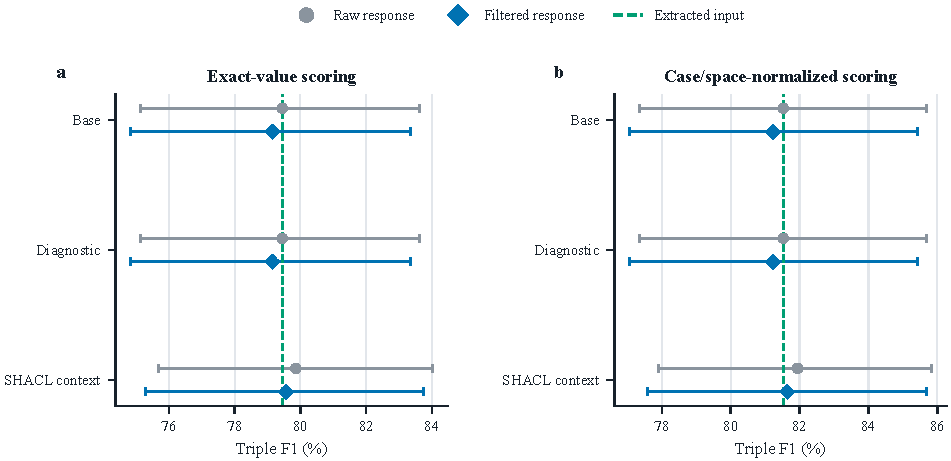
\includegraphics[width=0.98\textwidth]{figure/experiments/external_receipts.pdf}
\caption{首次收据评分。点表示平均 F1，误差线为 95\% 文档 bootstrap 置信区间。每个原始／过滤对照使用一个响应。虚线表示输入 F1。}
\label{fig:external_receipts}
\end{figure}
% End merged sections/external_receipts.tex

% Begin merged sections/reextraction_diagnostics.tex
\subsection{收据修复与重新抽取细节}
\label{app:reextraction_diagnostics}

我们在相同的 60 张新测试收据上再收集 240 个 Gemma 响应，比较有无索引下的修复与重新抽取。各设置共享来源行、字段含义、文档编号和输出上限；修复额外获得已有图。主分数差为过滤后的索引修复减索引重新抽取。全部 240 个响应的 JSON 都包含 Markdown 代码围栏。固定的严格解析器将其记为失败，各设置 F1 均为零。

采集后，我们去掉外层围栏，并执行相同模式检查。全部 240 个响应随即可解析。表~\ref{tab:reextraction_recovery}~给出这些补充评分。索引修复 F1 为 83.93\%，索引重新抽取为 61.05\%，配对差为 22.88 个百分点（95\% 置信区间：14.84 至 31.35）。

\begin{table}[t]
\centering
\caption{60 张收据在采集后的补充评分。围栏兼容处理去掉外层 Markdown 围栏。编号规范化还在过滤前分配已知文档编号。两者均使用保存的响应。}
\label{tab:reextraction_recovery}
\small
\begin{tabular}{lrrr}
\toprule
方法 & 围栏兼容 F1 & 编号规范化 F1 & 错误编号图数 \\
\midrule
重新抽取 & 0.6333 & 0.7256 & 18/60 \\
索引抽取 & 0.6105 & 0.7486 & 28/60 \\
修复率 & 0.7917 & 0.7917 & 0/60 \\
索引修复 & 0.8393 & 0.8393 & 0/60 \\
\bottomrule
\end{tabular}
\end{table}

索引重新抽取在 28 张图中给出错误文档编号；索引修复在全部 60 张图中使用正确编号。为四种设置统一分配已知编号后，索引重新抽取 F1 提高到 74.86\%，索引修复领先 9.07 个百分点（95\% 置信区间：5.22 至 13.10）。编号修正保持字段值不变。原来的 22.88 个百分点差距同时包含编号和字段值的影响。初始图构建成本与这些修复调用分别计算。

\paragraph{行索引覆盖的字段。}

我们在来源行中定位最初后续测试的 240 个参考字段。匹配保留大小写和标点，并清理空白。一个值跨越多行时，索引必须包含某次出现的全部行。240 个值中，188 个出现在索引行或邻近行，36 个出现在范围外，16 个与来源文本不同。对于覆盖的 188 个值，简单流程 精确返回 163 个，证据索引 返回 174 个。对于范围外的 36 个值，两者都返回 26 个；与来源不同的 16 个值，两者都未返回。索引净增加的十一项精确匹配来自覆盖组。

% Begin merged sections/call_policy_support.tex
\subsection{按可见错误调用修复}
\label{app:call_policy}

我们测试基于可见编号、关系、重复、字段数量和来源匹配错误的调用规则。它为每篇文档选择返回输入，或返回保存的修复输出。在 450 项模型构建与干净图混合流上，仅对 6.22\% 的输入调用修复，却漏掉 63.64\% 有参考差异的图。其 F1 为 94.46\%，始终调用修复为 95.82\%。可见检查漏掉许多缺失或字段分配错误的值。主方法对每篇文档都调用修复。

% Begin merged sections/offline_diagnostics.tex
\paragraph{早期选择器中的有用编辑。}

我们使用早期选择器保存的建议与试改图。这些运行早于表~\ref{tab:math_revision_selector}~中的共享特征和候选启动修改。对每篇文档，尝试模型编辑包的所有子集，并根据参考图为结果计分。执行保存编辑时关闭停止、成本和图边界检查。参考得分最高的子集称为 oracle。这项分析使用模型编辑包和参考值。

我们在 450 个输入上尝试 2,144 个子集，结果见表~\ref{tab:selection_bottlenecks}。注入缺陷输入中，86 张图未检测到违规，其中 72 张缺少参考字段，70 张存在能提高 F1 的建议子集。检查的试改中，212 项提高参考 F1，但效用分数不大于零。模型构建输入的对应数量为 8 张图和 1 项试改。

\begin{table}[t]
\centering
\caption{早期选择器结果，每组 225 个输入。oracle 利用参考答案寻找最佳保存子集。一篇文档可以有多次试改。}
\label{tab:selection_bottlenecks}
\small
\begin{tabular}{lrr}
\toprule
诊断项 & 受控输入 & 模型构建输入 \\
\midrule
预处理图 F1 & 0.8472 & 0.8799 \\
均匀选择器 F1 & 0.8472 & 0.8833 \\
固定建议 oracle F1 & 0.9964 & 0.9173 \\
初始未检出违规 & 86 & 198 \\
其中与参考不同的图 & 72 & 50 \\
其中存在可改善结果的图 & 70 & 8 \\
提高参考分数但效用非正的试改 & 212 & 1 \\
\bottomrule
\end{tabular}
\end{table}

去掉编辑成本使 67 篇注入缺陷文档的 F1 提高，158 篇不变，0 篇降低。模型构建输入中，0 篇提高，222 篇不变，3 篇降低。这三张图在清理后已经与参考不同。全部 148 个原本精确匹配的模型构建输入保留其 F1。注入缺陷输入的配对增益为 4.58 个百分点（95\% 文档 bootstrap 置信区间：3.69--5.54）。同一成本修改在两组输入上作用不同。


\subsection{图检查的时间与内存}
\label{sec:eval:scale}

我们在包含 1K--50K 条三元组的独立文档批次上，测量式~(\ref{eq:diagnostic_context})~中报告的耗时。完整扫描检查所有文档，局部更新只检查一篇已修改文档。完整扫描时间取七次运行的中位数，局部更新时间取 200 次运行的中位数，数值见表~\ref{tab:diagnostic_scaling}。内存统计构建批次时新增 Python 内存的峰值。源文本和模式对象共享，模型调用时间另计。

\begin{figure}[t]
\centering
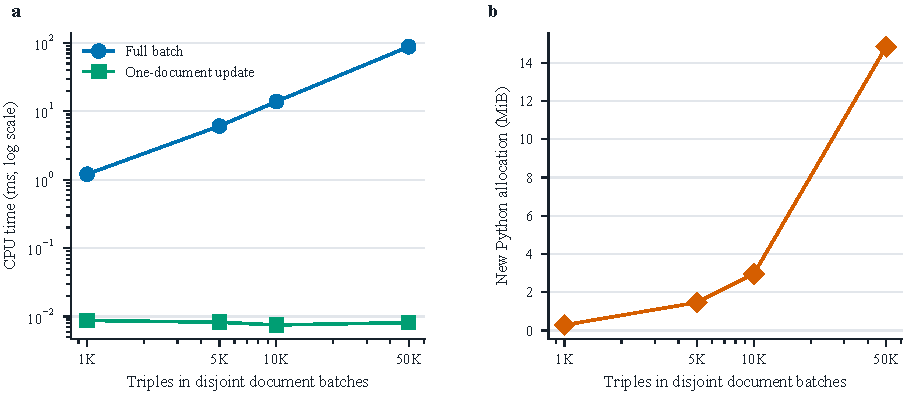
\includegraphics[width=0.98\textwidth]{figure/experiments/diagnostic_scaling.pdf}
\caption{独立文档批次的报告时间和内存。局部更新只检查一篇修改后的文档。内存统计共享源文本时新增的批次存储。}
\label{fig:diagnostic_scaling}
\end{figure}

\subsection{补充质量与抽取检查}
\label{sec:eval:external_benchmark}

Gemma 评判器在方法名称隐藏的条件下，为 180 个来源与三元组对打分。来源分数与精确参考有效性的 Pearson 相关系数为 $r=0.794$，Spearman 相关系数为 $\rho=0.807$（两者均有 $p<2.4\times10^{-40}$）。另外五次运行中，固定 50 项样本的均值都为 0.96。

我们在 45 篇均衡 TNEWS 文档上，将本文抽取器与 Neo4j Labs 的 \texttt{LLMGraphTransformer} 核心比较\citep{ref_neo4j_llm_graph_builder}。字段抽取器的类别准确率为 0.556，Graph Builder 为 0.533，配对检验为 $p=1.00$。

\subsection{请求成本与检查时间}
% Begin merged sections/audit_supporting.tex
\begin{table*}[t]
\centering
\caption{请求成本。平均时间包含重试和请求间隔等待。来源设置与排队时间另计。}
\label{tab:matched_cost}
\small
\resizebox{\textwidth}{!}{%
\begin{tabular}{llrrrr}
\toprule
输入 & 上下文 & 调用数 & 输入 token & 输出 token & 总耗时（秒） \\
\midrule
受控输入 & 基础提示 & 1.00 & 947 & 517 & 8.58 \\
受控输入 & 诊断提示 & 1.00 & 1017 & 512 & 8.61 \\
受控输入 & SHACL & 1.00 & 3080 & 513 & 8.45 \\
模型构建输入 & 基础提示 & 1.00 & 832 & 458 & 7.51 \\
模型构建输入 & 诊断提示 & 1.00 & 901 & 462 & 7.90 \\
模型构建输入 & SHACL & 1.00 & 2822 & 455 & 8.16 \\
\bottomrule
\end{tabular}%
}
\end{table*}
\begin{table*}[t]
\centering
\caption{图报告的时间和内存。内存统计新增批次存储峰值，单位为 MiB，源文本共享。}
\label{tab:diagnostic_scaling}
\small
\resizebox{\textwidth}{!}{%
\begin{tabular}{rrrrr}
\toprule
三元组 & 文档数 & 完整（毫秒） & 局部（毫秒） & 内存（MiB） \\
\midrule
1,000 & 143 & 1.20 & 0.009 & 0.29 \\
5,000 & 716 & 6.08 & 0.008 & 1.47 \\
10,000 & 1,434 & 13.90 & 0.008 & 2.96 \\
50,000 & 7,173 & 88.10 & 0.008 & 14.84 \\
\bottomrule
\end{tabular}%
}
\end{table*}
% End merged sections/audit_supporting.tex
